% Generated from data/prepared_demo_run.json and data/prepared_demo_evidence.json.
\resizebox{\columnwidth}{!}{%
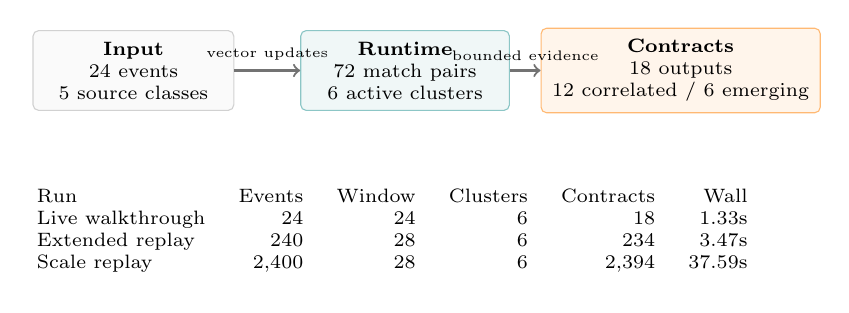
\begin{tikzpicture}[
  font=\scriptsize,
  box/.style={draw=black!18, rounded corners=2pt, fill=gray!4, inner sep=4pt, align=center},
  runbox/.style={draw=teal!45, rounded corners=2pt, fill=teal!6, inner sep=4pt, align=center},
  outbox/.style={draw=orange!55, rounded corners=2pt, fill=orange!8, inner sep=4pt, align=center},
  arrow/.style={->, thick, draw=black!55}
]
  \node[box, minimum width=2.55cm, minimum height=1.0cm] (input) at (0,2.8) {
    \textbf{Input}\\24 events\\5 source classes
  };
  \node[runbox, minimum width=2.65cm, minimum height=1.0cm] (runtime) at (3.45,2.8) {
    \textbf{Runtime}\\72 match pairs\\6 active clusters
  };
  \node[outbox, minimum width=2.75cm, minimum height=1.0cm] (contracts) at (6.95,2.8) {
    \textbf{Contracts}\\18 outputs\\12 correlated / 6 emerging
  };
  \draw[arrow] (input) -- node[above, font=\tiny] {vector updates} (runtime);
  \draw[arrow] (runtime) -- node[above, font=\tiny] {bounded evidence} (contracts);

  \node[anchor=north west, align=left] at (-1.35,1.45) {
    \begin{tabular}{@{}lrrrrr@{}}
      \toprule
      Run & Events & Window & Clusters & Contracts & Wall \\
      \midrule
    Live walkthrough & 24 & 24 & 6 & 18 & 1.33s \\
    Extended replay & 240 & 28 & 6 & 234 & 3.47s \\
    Scale replay & 2,400 & 28 & 6 & 2,394 & 37.59s \\
      \bottomrule
    \end{tabular}
  };
\end{tikzpicture}%
}
